%
% Meteoroid printable manual
%
% If you're a human, skip to "\mainmatter" to skip over the preamble.
%
\documentclass[10pt,twocolumn,openany,article]{memoir}

\setstocksize{9in}{6in}
\settrimmedsize{\stockheight}{\dimexpr 6in-15mm}{*}

\setlrmarginsandblock{.5cm}{1.5cm}{*}
\setulmarginsandblock{1.5cm}{*}{1}
\checkandfixthelayout


%% TV Standard

\ifdefined\TVNTSC
\newcommand\TV{NTSC}
\newcommand\REGION{US, Canada, Mexico, Brazil, and Japan}
\else
\ifdefined\TVPAL
\newcommand\TV{PAL}
\newcommand\REGION{UK and Europe (except France)}
\else
\ifdefined\TVSECAM
\newcommand\TV{SECAM}
\newcommand\REGION{France, Russia, Africa}
\else
\error{Must define a TV standard}
\fi
\fi
\fi


\usepackage[utf8]{inputenc}
\usepackage{babel}
\usepackage{stfloats}
\usepackage{microtype}
\usepackage{graphicx}
\usepackage{pdfpages}
\tolerance=1
\emergencystretch=\maxdimen
%\usepackage{tgtermes}
\usepackage{hyperref}
\usepackage{xcolor}
\hypersetup{
    colorlinks,
    linkcolor={red!50!black},
    citecolor={blue!50!black},
    urlcolor={blue!80!black},
    pdftitle={Meteoroid \ifdefined\DEMO{ Demo }\fi Manual for \TV},
    pdfsubject={Meteoroid videogame for the Atari 2600},
    pdfauthor={Bruce-Robert Pocock}%,
%    pdfkeywords={Your PDF keywords}
  }
\usepackage{caption}
\captionsetup{labelformat=empty}
\usepackage[protrusion=true,expansion=true]{microtype}
\fontfamily{pnc}
\chapterstyle{komalike}

\checkandfixthelayout

\title{Meteoroid \ifdefined\PLUSCART PlusCart \fi\ifdefined\DEMO Demo \fi Player's Guide}
\author{Bruce-Robert Pocock}


%%% BEGIN DOCUMENT

\begin{document}
\frontmatter
%%%\let\cleardoublepage\clearpage

\includepdf[height=9in,width=6in,fitpaper=true]{../Manual/Cover.png}

% \clearpage

% \maketitle

\thispagestyle{empty}

\twocolumn[

\chapter*{Introduction}\label{Introduction}

You've  just arrived  at Planet  Aaron. The  Galactic Police  are deeply
concerned  about a  meteoroid hijacked  by the  pirate faction  and have
hired you to investigate. It's quite  possible that the contents of this
meteoroid caused the destruction of the planet TS-499!

\bigskip

In  the \textit{Meteoroid}  videogame, you'll  move around  Planet Aaron
looking for  the meteoroid and its  contents. You'll have to  fight both
monsters from the local planet and pirates, and discover new weapons and
abilities to progress.

\vspace{2in}\vfill

This is the \textit{Meteoroid} \ifdefined\PLUSCART PlusCart \fi\ifdefined\DEMO Demo \fi Player's Guide

Copyright \copyright{} 2021, Bruce-Robert Pocock

\bigskip

This  version is  for systems  in \REGION{}  using the  \TV{} television
standard. For Atari  Video Computer System CX-2600  (or Sears Tele-Games
Video  Arcade or  Atari  7800 ProSystem),  \ifdefined\PLUSCART with  the
PlusCart,   and   \fi  optionally   with   AtariVox   (or  MemCard,   or
SaveKey) device.

\bigskip

This videogame software was not created, published, or licensed by Atari
or its successors.

\ifdefined\DEMO
\bigskip

This manual describes a \ifdefined\PLUSCART PlusCart \fi DEMO version of the game. The full version may
be different.
\fi

]

\let\cleardoublepage\clearpage

\mainmatter

\tableofcontents

\chapter{Setting Up}\label{Setting Up}

To play \textit{Meteoroid}, you will need:

\begin{itemize}
\item An Atari  console: the Atari Video Computer  System CX-2600, Sears
  Tele-Games  Video Arcade,  Atari  2600jr game  system,  or Atari  7800
  ProSystem
\item A TV or video display
\item        A        joystick         controller        (or        SEGA
  \ifdefined\TVNTSC{Genesis/}\fi{}MegaDrive                     gamepad)
\item (optional) A memory device: an AtariVox device with (optional) speakers or
  headphones, or a MemCard or SaveKey device.
  \ifdefined\PLUSCART
\item The PlusCart cartridge
  \else
\item The \textit{Meteoroid} game cartridge
  \fi
\end{itemize}

\begin{figure*}[b]
  \begin{center}
    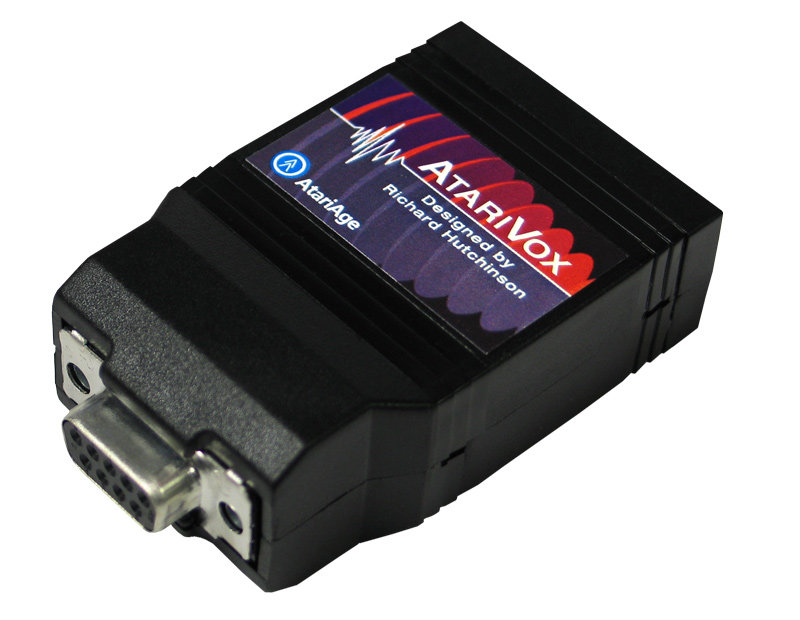
\includegraphics[width=\columnwidth]{../Manual/AtariVox.jpeg}
    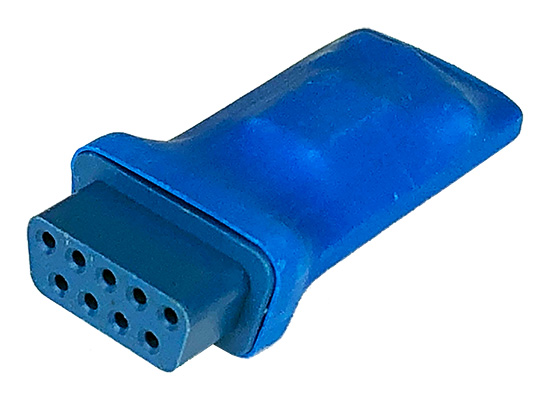
\includegraphics[width=\columnwidth]{../Manual/SaveKey.jpeg}
  \end{center}
\end{figure*}

Set up  your console with your  TV or video display.  Connect a joystick
controller  (or SEGA  \ifdefined\TVNTSC{Genesis/}\fi{}MegaDrive gamepad)
to  the \emph{left}  controller  port\ifdefined\PLUSCART\else{}. If  you
have  one, connect  your memory  device to  the \emph{right}  controller
port. Make  certain that the  Power switch is  in the Off  position when
connecting your memory device\fi{}.

Finally,     insert    the     \ifdefined\PLUSCART    PlusCart     \else
\textit{Meteoroid} game  cartridge (with the  label facing up)  \fi into
the cartridge slot, and turn the Power On.

\begin{figure}[h]
  \begin{center}
    \includegraphics[width=\columnwidth]{../Manual/Atari-2600-Wood-4Sw-Set.png}
  \end{center}
\end{figure}


\vfill

\chapter{How To Play}

\section{Console Controls}

\ifdefined\TVSECAM
\else

\ifdefined\TVPAL
\subsection{Colour/B\&W Switch (Pause)}

On an  Atari 2600  (or Sears Arcade)  you can pause  the game  using the
\textbf{Colour/B\&W Switch}.  Push the \textbf{Colour/B\&W}  switch into
the \textbf{Colour} position  to play, or the  \textbf{B\&W} position to
pause the game.

\ifdefined\PLUSCART\else
On the  Atari 7800, press  the \textbf{Pause}  button once to  pause the
game, and again to resume playing.
\fi

\else

\subsection{Color/B\&W Switch (Pause)}

On an  Atari 2600  (or Sears Arcade)  you can pause  the game  using the
\textbf{Color/B\&W Switch}. Push the \textbf{Color/B\&W} switch into the
\textbf{Color} position to play, or the \textbf{B\&W} position to pause the game.

\ifdefined\PLUSCART\else
On the  Atari 7800, press  the \textbf{Pause}  button once to  pause the
game, and again to resume playing.
\fi

\fi
\fi

\subsection{Game Select}

When  viewing the  Title Screen,  you can  use the  \textbf{Game Select}
switch to choose the Slot you wish to use to save your progress.

While you  are playing the  game, you  can use the  \textbf{Game Select}
switch to review your current status.

\subsection{Game Reset}

When  viewing the  Select  Slot screen,  press  the \textbf{Game  Reset}
switch to begin playing the game.

While you are playing the game,  press the \textbf{Game Reset} switch to
abandon your progress and return to  the Title Screen. You will lose any
progress since the last time you saved your progress.

\subsection{Difficulty Switches}

You cannot delete a game in progress unless both Difficulty Switches are
in the  ``A'' (Advanced or Expert)  position. To protect your  game from
being deleted,  set either one of  the Difficulty Switches to  the ``B''
(Beginner or Novice) position.

\ifdefined\TVSECAM

The Left Difficulty Switch  can be used to pause game  play. When in the
``A'' (Advanced  or Expert) position, you  will not be able  to continue
playing  until  you  toggle  the   switch  to  the  ``B''  (Beginner  or
Novice) position.

\else

This  game does  not  make  use of  the  Difficulty  Switches while  you
are playing. 

\fi

\section{Using a Gamepad}

A   SEGA  \ifdefined\TVNTSC{Genesis/}\fi{}MegaDrive   gamepad  (or   other
compatible controller) may also be used with \textit{Meteoroid}. Use the
\textbf{B} button  as the \textbf{Fire} button.  Use the \textbf{C} button  as an
alternative way to \textbf{Jump} switch.

Your gamepad must be plugged in before you turn on the power if you want
to use it. Otherwise, the \textbf{C} button will be ignored.

\section{Start a Game}

\begin{center}
  \includegraphics[width=\columnwidth]{../Manual/TitleAquax\TV.png}
\end{center}

Once your  console is set  up and everything  is connected, turn  on the
Power  switch. You'll  see  the  title screen  appear.  If  you have  an
AtariVox device, you'll also hear the title spoken.


\begin{center}
  \includegraphics[width=\columnwidth]{../Manual/SelectSlot\TV.png}
\end{center}

Press the \textbf{Game Select} switch or \textbf{Fire} button to move to
the Select Slot screen.

Press  the \textbf{Game  Select} switch  or move  the joystick  left and
right to choose a memory slot for your game. \ifdefined\PLUSCART

There are 3 memory slots possible if you have a memory device connected,
numbered  slot ``1''  through ``3.''  In addition,  you can  choose from
a Cloud Save slot,  with one of the letters ``A''  through ``C.'' If you
do not  have a memory  device connected, you  will only see  slots ``A''
through ``C'' available.

\else

There are 3 memory slots possible if you have a memory device connected,
numbered slot  ``1'' through ``3.'' If  you do not have  a memory device
connected, you  will see only  slot ``0,''  which does not  allow saving
your progress once the power is turned off.

\fi

Press \textbf{Game Select} or the  joystick left/right to rotate through
them.  If  someone  has  already begun  to  play  \textit{Meteoroid}  in
a certain slot, your screen will  show ``\texttt{RESUME}.'' If a slot is
empty, you'll see ``\texttt{BEGIN}'' instead.

\ifdefined\DEMO
\skip
This  demo  saves your  progress  in  the  ``scratchpad'' area  of  your
memory  device.  It's possible  that  other  games might  overwrite  and
destroy your saved progress. This is  just because it's a demo, and does
not have a private area reserved for it.
\ifdefined\PLUSCART
This demo  also saves to  a different cloud  storage area than  the full
game will do.  Save game slots ``A'' through ``C''  are distinct for the
demo versus the full game.
\fi
\skip
\fi

When you have selected the slot you want to begin (or resume), press the
\textbf{Game Reset} switch or \textbf{Fire} button to start.

\fi

You'll begin at your space ship on the surface of Planet Aaron.

\section{Exploring Planet Aaron}

Use the joystick controller to walk to the left or right. To jump, press
the   joystick   controller  up\footnote{or   press   the  ``C''   button   on
a  Genesis/MegaDrive  control  pad}.  To fire  your  weapon,  press  the
\textbf{Fire} button. 

\section{Game Over}

If  you fail  in your  mission,  your game  is over.  However, you  have
another chance to continue.

\begin{figure}[b]
  \begin{center}
    \includegraphics[width=\columnwidth]{../Manual/GameOver\TV.png}
  \end{center}
\end{figure}

When you continue, it'll  be just as if you'd never  failed in the first
place. However,  you'll start  over from  the last  Save Point  that you
encountered in the game

Just  choose   your  game   slot  from  the   Title  Screen   to  resume
your adventure.

\section{Winning the Game}

...

\section{Starting Over}\label{Starting Your Adventure Over}

When you choose a  slot with no game record in  it already, you'll begin
a new adventure.

If you want to delete your adventure  and start again, it's a little bit
tricky. This is to make sure you don't accidentally lose your progress!

From the  Title Screen, press  \textbf{Game Select} or the  \textbf{Fire} button.
Then, press  \textbf{Game Select}  or move the  joystick left  and right
until the slot you want to erase is shown.

Here's the tricky part. You'll need to:

\begin{itemize}
\item Make sure that both of the Difficulty Switches on your console
  are set to the ``A'' (Advanced or Expert) position.
\item With your joystick controller, pull down (toward you) on the
  joystick and hold down the \textbf{Fire} button.
\end{itemize}

The screen  will change from  saying ``\texttt{SELECT SLOT}''  to saying
``\texttt{ERASE  SLOT}.''   The  text   will  also   be  red   to  catch
your attention.

If  you're  \emph{sure}   you  want  to  erase  your   game  data,  then
\emph{without}  letting go  of the  \textbf{Fire}  button, move  the joystick  up
(toward  the TV).  You'll see  that the  slot changes  from ``\texttt{IN
  USE}'' to ``\texttt{VACANT}'' \emph{immediately}.

\emph{Once your game record has been erased, you can not recover it from
  the game, so think carefully before you erase it.}

\subsection{Protecting Your Game Record}

If  either of  your Difficulty  Switches is  in the  ``B'' (Beginner  or
Novice) position, then you can't erase  a game slot. \emph{Tip: When you
  connect your memory device, check the position of those switches.}

\ifdefined\TVSECAM

Remember,  the  Left  Difficulty  Switch  is used  to  pause  the  game.
After deleting your save game slot, return the Left Difficulty Switch to
the ``B'' position.

\fi

\fi % not-nosave

\chapter{Troubleshooting}

\ifdefined\DEMO

\section{Screen ``Jitters,'' freezes,  \ifdefined\TVPAL appears in black
  \& white,\fi or flashes blue}

These may  be signs that  a screen  (or the transition  between screens)
does not have the correct ``scan line'' count. This is a technical error
by the game's  developer (that's me!) and must be  surecorrected in the next
version of the game.

\ifdefined\TVPAL
If the  picture is in  black-and-white throughout, make sure  you're not
running the SECAM version.
\fi

If you see these effects (or if you are running in Stella, if you notice
that the scan  line count is not \ifdefined\TVNTSC 262  \else 312 \fi at
all         times)         please         report         them         to
\hred{mailto:support@star-hope.org}{support@star-hope.org} so  that they
can be corrected before the game is finished.

\fi

\section{Sad Face Screen}

If you  see the Sad  Face screen,  the game is  trying to tell  you that
there is a problem.

From here, you can press the \textbf{Game Reset} switch to return to the
Title Screen.

\ifdefined\PLUSCART\else

\includegraphics[width=\columnwidth]{../Manual/WhiteSadFace\TV.png}

The white sad  face screen means that the game  has encountered an error
and cannot continue. 

You  should   not  be  able   to  reach  this  screen.   Please  contact
\href{mailto:support@star-hope.org}{support@star-hope.org}           for
additional assistance. Send the code  number that appears on this screen
with your email.

\section{Pause button must be held down (7800)}

This  is believed  to  be  a side  effect  of  certain multi-carts,  eg.
PlusCart.   If  you   are  encountering   this  problem,   please  check
\href{https://github.com/brpocock/grizzards/issues/182}{https://\-github.com/\-brpocock/\-grizzards/\-issues/\-182}
for current information.

Note  that you  can  press  \textbf{Game Select}  to  view your  current
progress and effectively pause the game as well.

\section{TV goes blank at Save Point}

\ifdefined\PLUSCART
If you are saving to a local memory device (slot ``1'' through ``3''), make
\else
Make
\fi
sure your memory device is  connected. If your memory device is not
connected when the game tries to save, you may see the TV picture remain
blank while the game tries to record your progress.

\section{No voices}

When the game first starts the title screen, after a brief pause, you'll
hear the AtariVox announce the name of the game. If you don't, make sure
that  the AtariVox  is connected  and the  speakers (or  headphones) are
connected, powered on, and turned up.

Naturally, there are no voices if you do not have an AtariVox device.

\fi

\chapter{Technical Notes}

The following notes are of interest to hackers only. You don't need to
understand anything in this section to play \textit{Meteoroid}.

\section{Development Tools}

The \textit{Meteoroid} source code and development tools are available from
\href{https://Star-Hope.org/games/Meteoroid/}{https://Star-Hope\-.org/\-games/\-Meteoroid/} 
the \textit{Meteoroid} web site.

\section{Game Record Slots}

There are 3  logical game slots that  you can choose from  for the game.
Each save game slot takes up 1 block (64 bytes) of storage space on your
memory device, for  a total of 3  blocks for all three  save game slots.
The following blocks are used:

\ifdefined\PLUSCART

Save  Game slots  ``A,''  ``B,''  and ``C''  are  ``cloud'' save  slots.
The  contents of  these slots  are saved  to the  \textit{Meteoroid} web
server and accessed over the WiFi link in your PlusCart.

\fi

\ifdefined\DEMO

\begin{enumerate}
\item block \$cc (addresses \$3300-\$333f)
\item block \$cd (addresses \$3340-\$337f)
\item block \$ce (addresses \$3380-\$33bf)
\end{enumerate}

These blocks are in the Scratchpad  area. This means that other programs
might potentially disrupt or destroy your saved game record.

The final version of this game will use a different set of memory blocks
that  are  reserved   for  its  own  private  use,  so   this  won't  be
a problem then.

\else

\begin{enumerate}
\item block \$41 (addresses \$1040-\$107f)
\item block \$42 (addresses \$1080-\$10bf)
\item block \$43 (addresses \$10c0-\$10ff)
\end{enumerate}

The addresses  used by the Save  Game Slots are NOT  YET registered with
AtariAge, so they won't OR MAYBE  WILL conflict with any other games you
might play.

A deleted game  on your memory device can sometimes  be recovered if you
have a  Harmony, PlusCart, or Uno  cartridge, or a similar  cartridge to
which  you can  upload  a ROM  file.  Visit the  Meteoroid  web site  at
\href{https://Star-Hope.org/games/Meteoroid/}{https://Star-Hope\-.org/\-games/\-Meteoroid/}
and download the  Unerase utility program. If you have  just erased your
game's progress, you can probably recover it.

\ifdefined\PLUSCART
A deleted game from your ``cloud'' save games cannot be recovered.
\fi

\fi


\subsection{Portability}

The save game records are in the same format for all \textit{Meteoroid} game
cartridges, regardless of the region for which they were saved.  This means
that you can save your progress on an NTSC type system and then continue
playing on a PAL or SECAM system, or vice-versa.

\ifdefined\DEMO

The save  game slots used by  this demo, however, are  distinct from the
ones that will be used in the final game.

\fi

\chapter{Credits}

{\small

  The  \textit{Meteoroid} videogame  software,  including its  audiovisual
components   and  this   manual,   are   copyright  \copyright{}   2021,
Bruce-Robert  Pocock.   All  Rights  are  Reserved   except  as  granted
under license.

\begin{itemize}
\item Bruce-Robert Pocock --- Programming, Manual text, In-Game Artwork,
  Sound effects
\item Zephyr Salz --- Art for manual, label, and cover; Music
\end{itemize}

\bigskip


Includes VCS  header file by  Matthew Dillon, Olaf  ``Rhialto'' Seibert,
Andrew  Davie, and  Peter H.  Froehlich. Binary  to decimal  translation
based upon  code by  Andrew Jacobs,  based upon  code by  Garth Wilsone.
``Six  Digit Score''  48 pixel  wide  display routines  as explained  on
Stella list  by Erik  Mooney and  Bradford W.  Mott. SaveKey  EEPROM and
AtariVox  speech  synthesis driver  based  upon  code by  Alex  Herbert.
Random  number  generator  by  AtariAge  forum  user  \texttt{Supercat}.
Some  math  functions  by AtariAge  forum  user  \texttt{Omega\-matrix}.
Some  math functions  taken  from December  1984 \textit{Apple  Assembly
  Line}.  ``Have  You   Played  Atari  Today''  jingle   by  Atari  Inc.
transcribed by AtariAge Forum user \texttt{tigger\-the\-hun}. Atari 7800
console  detection logic  by AtariAge  user \texttt{batari}  courtesy of
Darrell Spice, Jr. AtariVox and SaveKey illustrations in this manual are
from  the AtariAge  store.  \ifdefined\DEMO\else The  AtariAge logo  and
logotype are the property of AtariAge. \fi

Special thanks  to everyone in  the Stella and AtariAge  communities for
making this game possible.

\subsection{Testers}


This section will list anyone who helps to playtest this game. ***

}


\vfill

\chapter*{Publication History}

The \textit{Meteoroid} videogame software has not yet been published.

It is ``alpha'' quality software.

A  demo version  was created  in September,  2021. \ifdefined\DEMO  This
manual describes that demo. \fi

\subsection{License}

You are hereby granted permission  to make use of the \textit{Meteoroid}
videogame software for \emph{non-commercial personal use}.

Redistribution not for profit is allowed, but sales of this software
requires a license.

\end{document}
